% questions.tex —— 1987 年·全国卷·理科 · 题目内容片段（无答案）
% 由 tools/generate_projects.py 依来源总账自 1987/1987_数学真题_全国理_试题.md 生成，勿手改（改源 MD 后重跑）


\gkpart{理科数学}

\begin{gktip}
\textbf{来源说明}：本题面依据固定源 PDF《1987 普通高等学校招生考试（全国卷理）》逐题转录。固定源 PDF 共 1 页、原卷印刷页码 30；该 PDF 不含答案和解析页，下列答案和解析由本库独立推导，不声称代表官方发布版本。

\textbf{图形说明}：第 6 题的正弦曲线、第 8 题的四个图象选项和第 17 题的三棱锥图依据固定源图形关系重绘为 TikZ 矢量图。
\end{gktip}

\begin{question}
\gkti{1}设 $S,T$ 是两个非空集合，且 $S\nsubseteq T,\ T\nsubseteq S$，令 $X=S\cap T$，那么 $S\cup X$ 等于\mbox{（　　）}

（A）$X$　　（B）$T$　　（C）$\varnothing$　　（D）$S$

\end{question}
\begin{question}
\gkti{2}设椭圆方程为

\nopagebreak[4]
\[
\frac{x^2}{a^2}+\frac{y^2}{b^2}=1\qquad(a>b>0),
\]

令 $c=\sqrt{a^2-b^2}$，那么它的准线方程为\mbox{（　　）}

（A）$y=\pm\dfrac{a^2}{c}$　　（B）$y=\pm\dfrac{b^2}{c}$

（C）$x=\pm\dfrac{a^2}{c}$　　（D）$x=\pm\dfrac{b^2}{c}$

\end{question}
\begin{question}
\gkti{3}设 $a,b$ 是满足 $ab<0$ 的实数，那么\mbox{（　　）}

（A）$|a+b|>|a-b|$　　（B）$|a+b|<|a-b|$

（C）$|a-b|<\bigl||a|-|b|\bigr|$　　（D）$|a-b|<|a|+|b|$

\end{question}
\begin{question}
\gkti{4}已知 $E,F,G,H$ 为空间中的四个点，设命题甲：点 $E,F,G,H$ 不共面；命题乙：直线 $EF$ 和 $GH$ 不相交。那么\mbox{（　　）}

（A）甲是乙的充分条件，但不是必要条件

（B）甲是乙的必要条件，但不是充分条件

（C）甲是乙的充要条件

（D）甲不是乙的充分条件，也不是乙的必要条件

\end{question}
\begin{question}
\gkti{5}在区间 $(-\infty,0)$ 上为增函数的是\mbox{（　　）}

（A）$y=-\log_{\frac12}(-x)$　　（B）$y=\dfrac{x}{1-x}$

（C）$y=-(x+1)^2$　　（D）$y=1+x^2$

\Needspace{0.4\textheight}
\end{question}
\begin{question}
\gkti{6}要得到函数

\nopagebreak[4]
\[
y=\sin\left(2x-\frac\pi3\right)
\]

的图象，只需将函数 $y=\sin2x$ 的图象（如图）\mbox{（　　）}
\nopagebreak[4]
\begin{center}% 1987 年全国卷理科第 6 题：y=sin 2x 图象
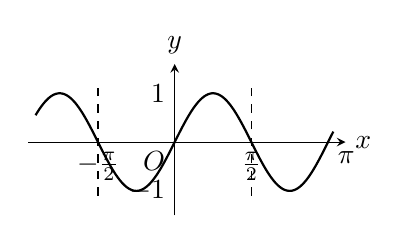
\begin{tikzpicture}[scale=0.62,>=stealth]
  \draw[->] (-3.0,0)--(3.5,0) node[right] {$x$};
  \draw[->] (0,-1.5)--(0,1.6) node[above] {$y$};
  \draw[thick,domain=-2.85:3.25,samples=160]
    plot (\x,{sin(114.592*\x)});
  \draw[dashed] (-1.57,-1.1)--(-1.57,1.1);
  \draw[dashed] (1.57,-1.1)--(1.57,1.1);
  \node[below] at (-1.57,0) {$-\frac\pi2$};
  \node[below] at (1.57,0) {$\frac\pi2$};
  \node[below right] at (3.14,0) {$\pi$};
  \node[left] at (0,1) {$1$};
  \node[left] at (0,-1) {$-1$};
  \node[below left] at (0,0) {$O$};
\end{tikzpicture}
\end{center}
\nopagebreak[4]
（A）向左平行移动 $\dfrac\pi3$　　（B）向右平行移动 $\dfrac\pi3$

（C）向左平行移动 $\dfrac\pi6$　　（D）向右平行移动 $\dfrac\pi6$

\end{question}
\begin{question}
\gkti{7}极坐标方程

\nopagebreak[4]
\[
\rho=\sin\theta+2\cos\theta
\]

所表示的曲线是\mbox{（　　）}

（A）直线　　（B）圆　　（C）双曲线　　（D）抛物线

\Needspace{0.4\textheight}
\end{question}
\begin{question}
\gkti{8}函数

\nopagebreak[4]
\[
y=\arccos(\cos x)\qquad x\in\left[-\frac\pi2,\frac\pi2\right]
\]

的图象是\mbox{（　　）}
\nopagebreak[4]
\begin{center}% 1987 年全国卷理科第 8 题：y=arccos(cos x) 在 [-pi/2,pi/2] 上的四个图象选项
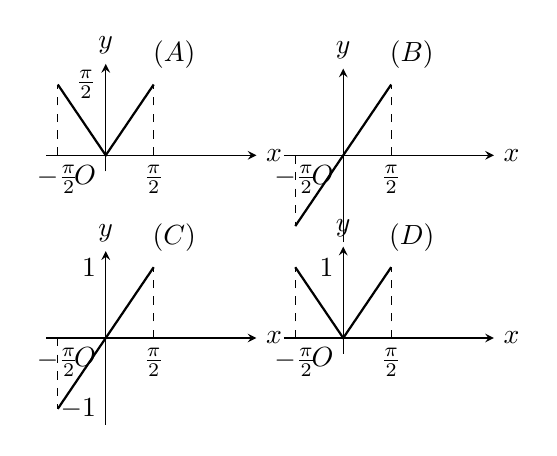
\begin{tikzpicture}[scale=0.58,>=stealth]
  \node at (1.5,2.2) {$(A)$};
  \draw[->] (-1.3,0)--(3.3,0) node[right] {$x$};
  \draw[->] (0,-0.35)--(0,2.0) node[above] {$y$};
  \draw[thick] (-1.05,1.55)--(0,0)--(1.05,1.55);
  \draw[dashed] (-1.05,0)--(-1.05,1.55) (1.05,0)--(1.05,1.55);
  \node[below] at (-1.05,0) {$-\frac\pi2$};
  \node[below] at (1.05,0) {$\frac\pi2$};
  \node[left] at (0,1.55) {$\frac\pi2$};
  \node[below left] at (0,0) {$O$};

  \begin{scope}[xshift=5.2cm]
    \node at (1.5,2.2) {$(B)$};
    \draw[->] (-1.3,0)--(3.3,0) node[right] {$x$};
    \draw[->] (0,-1.9)--(0,1.9) node[above] {$y$};
    \draw[thick] (-1.05,-1.55)--(1.05,1.55);
    \draw[dashed] (-1.05,0)--(-1.05,-1.55) (1.05,0)--(1.05,1.55);
    \node[below] at (-1.05,0) {$-\frac\pi2$};
    \node[below] at (1.05,0) {$\frac\pi2$};
    \node[below left] at (0,0) {$O$};
  \end{scope}

  \begin{scope}[yshift=-4.0cm]
    \node at (1.5,2.2) {$(C)$};
    \draw[->] (-1.3,0)--(3.3,0) node[right] {$x$};
    \draw[->] (0,-1.9)--(0,1.9) node[above] {$y$};
    \draw[thick] (-1.05,-1.55)--(1.05,1.55);
    \draw[dashed] (-1.05,0)--(-1.05,-1.55) (1.05,0)--(1.05,1.55);
    \node[below] at (-1.05,0) {$-\frac\pi2$};
    \node[below] at (1.05,0) {$\frac\pi2$};
    \node[left] at (0,1.55) {$1$};
    \node[left] at (0,-1.55) {$-1$};
    \node[below left] at (0,0) {$O$};
  \end{scope}

  \begin{scope}[xshift=5.2cm,yshift=-4.0cm]
    \node at (1.5,2.2) {$(D)$};
    \draw[->] (-1.3,0)--(3.3,0) node[right] {$x$};
    \draw[->] (0,-0.35)--(0,2.0) node[above] {$y$};
    \draw[thick] (-1.05,1.55)--(0,0)--(1.05,1.55);
    \draw[dashed] (-1.05,0)--(-1.05,1.55) (1.05,0)--(1.05,1.55);
    \node[below] at (-1.05,0) {$-\frac\pi2$};
    \node[below] at (1.05,0) {$\frac\pi2$};
    \node[left] at (0,1.55) {$1$};
    \node[below left] at (0,0) {$O$};
  \end{scope}
\end{tikzpicture}
\end{center}
\nopagebreak[4]
\end{question}
\begin{question}
\gkti{9}求函数

\nopagebreak[4]
\[
y=\tan\frac{2x}{3}
\]

的周期。

\end{question}
\begin{question}
\gkti{10}已知方程

\nopagebreak[4]
\[
\frac{x^2}{2+\lambda}-\frac{y^2}{1+\lambda}=1
\]

表示双曲线，求 $\lambda$ 的范围。

\end{question}
\begin{question}
\gkti{11}若 $(1+x)^n$ 的展开式中，$x^3$ 的系数等于 $x$ 的系数的 7 倍，求 $n$。

\end{question}
\begin{question}
\gkti{12}求极限

\nopagebreak[4]
\[
\lim_{n\to\infty}\left(
\frac1{n^2+1}+\frac2{n^2+1}+\frac3{n^2+1}
+\cdots+\frac{2n}{n^2+1}
\right).
\]

\end{question}
\begin{question}
\gkti{13}在抛物线 $y=4x^2$ 上求一点，使该点到直线 $y=4x-5$ 的距离为最短。

\end{question}
\begin{question}
\gkti{14}由数字 $1,2,3,4,5$ 组成没有重复数字且数字 1 与 2 不相邻的五位数。求这种五位数的个数。

\end{question}
\begin{question}
\gkti{15}一个正三棱台的下底和上底的周长分别为 $30\text{ cm}$ 和 $12\text{ cm}$，而侧面积等于两底面积之差，求斜高。

\end{question}
\begin{question}
\gkti{16}求

\nopagebreak[4]
\[
\sin10^\circ\sin30^\circ\sin50^\circ\sin70^\circ
\]

的值。

\Needspace{0.4\textheight}
\end{question}
\begin{question}
\gkti{17}如图，三棱锥 $P-ABC$ 中，已知 $PA\perp BC,\ PA=BC=L$，$PA,BC$ 的公垂线 $ED=h$。求证：三棱锥 $P-ABC$ 的体积

\nopagebreak[4]
\[
V=\frac16L^2h.
\]
\nopagebreak[4]
\begin{center}% 1987 年全国卷理科第 17 题：三棱锥及公垂线
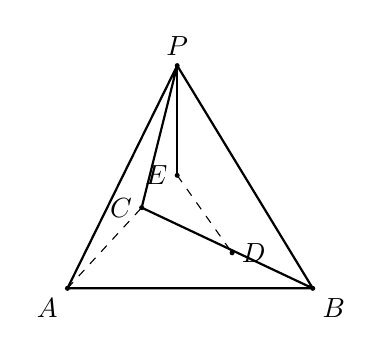
\begin{tikzpicture}[scale=0.82,>=stealth]
  \coordinate (P) at (1.7,3.45);
  \coordinate (A) at (0,0);
  \coordinate (B) at (3.8,0);
  \coordinate (C) at (1.15,1.25);
  \coordinate (E) at (1.7,1.75);
  \coordinate (D) at (2.55,0.55);
  \draw[thick] (P)--(A) (P)--(B) (P)--(C) (A)--(B) (B)--(C);
  \draw[dashed] (A)--(C) (E)--(D);
  \draw[thick] (E)--(P);
  \fill (P) circle (1.1pt) node[above] {$P$};
  \fill (A) circle (1.1pt) node[below left] {$A$};
  \fill (B) circle (1.1pt) node[below right] {$B$};
  \fill (C) circle (1.1pt) node[left] {$C$};
  \fill (E) circle (1.1pt) node[left] {$E$};
  \fill (D) circle (1.1pt) node[right] {$D$};
\end{tikzpicture}
\end{center}
\nopagebreak[4]
\end{question}
\begin{question}
\gkti{18}设对所有实数 $x$，不等式

\nopagebreak[4]
\[
x^2\log_2\frac{4(a+1)}a
+2x\log_2\frac{2a}{a+1}
+\log_2\frac{(a+1)^2}{4a^2}>0
\]

恒成立，求 $a$ 的取值范围。

\end{question}
\begin{question}
\gkti{19}设复数 $z_1$ 和 $z_2$ 满足关系式

\nopagebreak[4]
\[
z_1\overline{z_2}+\overline A z_1+A\overline{z_2}=0,
\]

其中 $A$ 为不等于 0 的复数。证明：

\Needspace{5\baselineskip}
（1） 证明：

\nopagebreak[4]
\[
|z_1+A||z_2+A|=|A|^2\text{；}
\]

\Needspace{5\baselineskip}
（2） 证明：

\nopagebreak[4]
\[
\frac{z_1+A}{z_2+A}
=\left|
\frac{\overline{z_1}+\overline A}
{\overline{z_2}+\overline A}
\right|\text{。}
\]

\end{question}
\begin{question}
\gkti{20}设数列 $a_1,a_2,\ldots,a_n,\ldots$ 的前 $n$ 项的和 $S_n$ 与 $a_n$ 的关系是

\nopagebreak[4]
\[
S_n=-ba_n+1-\frac{1}{(1+b)^n},
\]

其中 $b$ 是与 $n$ 无关的常数，且 $b\ne-1$。

（1） 求 $a_n$ 和 $a_{n-1}$ 的关系式；

（2） 写出用 $n$ 和 $b$ 表示 $a_n$ 的表达式；

\Needspace{5\baselineskip}
（3） 当 $0<b<1$ 时，求极限

\nopagebreak[4]
\[
\lim_{n\to\infty}S_n.
\]

\end{question}
\begin{question}
\gkti{21}定长为 $3$ 的线段 $AB$ 的两端点在抛物线

\nopagebreak[4]
\[
y^2=x
\]

上移动，记线段 $AB$ 的中点为 $M$，求点 $M$ 到 $y$ 轴的最短距离，并求此时点 $M$ 的坐标。

\end{question}
\gkpart{附加题}

\begin{question}
\gkti{22}求极限

\nopagebreak[4]
\[
\lim_{n\to\infty}\left(1-\frac1{2x}\right)^x.
\]

\begin{gktip}
\textbf{转录疑点}：原卷此处极限下标写 $n\to\infty$，但括号中的变量和指数写作 $x$；本题按固定源字面照录，未擅自把 $x$ 改成 $n$。
\end{gktip}

\end{question}
\begin{question}
\gkti{23}设

\nopagebreak[4]
\[
y=x\ln(1+x^2),
\]

求 $y'$。

\end{question}